\documentclass[nofootinbib,prd,superscriptaddress,twocolumn]{revtex4}
\usepackage{amsmath,graphicx,hyperref}
\usepackage{slashed}
\usepackage{feynmp}
\usepackage{epstopdf}
\usepackage{color}
\usepackage[dvipsnames]{xcolor}


%%%%%%%%%%%%%%%%%%%%%%%%%%%%%%%%%%%%%%%%%%%%%%%%%%%%%%%%%%%%%%%%%%%%%%
%%%%%%%%%%%%%%%%%%%%%%%%%%%%% Command %%%%%%%%%%%%%%%%%%%%%%%%%%%%%%%%
%%%%%%%%%%%%%%%%%%%%%%%%%%%%%%%%%%%%%%%%%%%%%%%%%%%%%%%%%%%%%%%%%%%%%%

\newcommand{\fms}[1]{{#1}\!\!\!/}
\newcommand{\fmsl}[1]{{#1}\!\!\!\!/}

\newcommand{\mc}{\mathcal}
\newcommand{\mr}{\mathrm}
\newcommand{\mP}{\mathcal{P}}
\newcommand{\mO}{\mathcal{O}}

\newcommand{\be}{\begin{equation}} 
\newcommand{\ee}{\end{equation}} 
\newcommand{\beq}{\begin{equation}} 
\newcommand{\eeq}{\end{equation}} 
\newcommand{\bea}{\begin{eqnarray}} 
\newcommand{\eea}{\end{eqnarray}} 

\newcommand{\ov}{\overline}
\newcommand{\pp}{\perp}
\newcommand{\dg}{\dagger}
\newcommand{\n}{\overline{n}}
\newcommand{\nn}{\frac{\fms{\overline{n}}}{2}} 
\newcommand{\nnn}{\frac{\fms{n}}{2}} 

\newcommand{\bl}[1]{{\bf{#1}}}
\newcommand{\bla}[1]{|{\bf{#1}}|}
\newcommand{\blp}[1]{{\bf{#1}}_{\perp}}
\newcommand{\blpu}[1]{{\bf{#1}}^{\perp}}
\newcommand{\blpa}[1]{|{\bf{#1}}_{\perp}|}
\newcommand{\bs}[1]{\boldsymbol{#1}}
\newcommand{\bsp}[1]{{\boldsymbol{#1}}_{\perp}}

\newcommand{\ds}{\displaystyle} 
\newcommand{\nnb}{\nonumber} 

\newcommand{\as}{\alpha_s}
\newcommand{\qa}{q_{A'}}

\newcommand{\eps}{\varepsilon} 
\newcommand{\veps}{\varepsilon} 

\newcommand{\UV}{\veps_{\mr{UV}}}
\newcommand{\IR}{\veps_{\mr{IR}}}

\newcommand{\La}{\Lambda^2_{\rm{alg}}}

%--- journals
\newcommand{\physrep}{Phys. Reports}
\newcommand{\mnras}{Mon. Not. R. Astron. Soc.}
\newcommand{\apjl}{Astrophys. J. Lett.}
\newcommand{\jcap}{J. Cosmol. Astropart. Phys.}

%--- for comments
\newcommand{\arz}[1]{{{\bf{\color{BrickRed}[ARZ: #1]}}}}

%%%%%%%%%%%%%%%%%%%%%%%%%%%%%%%%%%%%%%%%%%%%%%%%%%%%%%%%%%%%%%%%%%%%%%

\bibliographystyle{apsrev}

%\topmargin 0.0 in

\begin{document}

\baselineskip 3.0ex 

\vspace*{18pt}

%%%%%%%%%%%%%%%%%%%%%%%%%%%%%%%%%%%%%%%%%%%%%%%%%%%%%%%%%%%%%%%%%%%%%%
%%%%%%%%%%%%%%%%%%%%%%%%%%%%% Title %%%%%%%%%%%%%%%%%%%%%%%%%%%%%%%%%%
%%%%%%%%%%%%%%%%%%%%%%%%%%%%%%%%%%%%%%%%%%%%%%%%%%%%%%%%%%%%%%%%%%%%%%

\title{Updated Constraints on Self-Interacting Dark Matter from Supernova 1987A}

\def\Pitt{Pittsburgh Particle Physics Astrophysics and Cosmology Center (PITT PACC) \\ Department of Physics and Astronomy, University of Pittsburgh, Pittsburgh, Pennsylvania 15260, USA}

\author{Cameron Mahoney}
\email[E-mail:]{cbm34@pitt.edu}
\affiliation{\Pitt}
\author{Adam K. Leibovich}
\email[E-mail:]{akl2@pitt.edu}
\affiliation{\Pitt}
\author{Andrew R. Zentner}
\email[E-mail:]{zentner@pitt.edu}
\affiliation{\Pitt}  

\begin{abstract} 
\baselineskip 3.0ex   
Abstract?
\end{abstract}

\maketitle 

%%%%%%%%%%%%%%%%%%%%%%%%%%%%%%%%%%%%%%%%%%%%%%%%%%%%%%%%%%%%%%%%%%%%%%

%------------------------- Introduction ---
\section{Introduction}

A nearly overwhelming preponderance of observational evidence indicates that a form of nonrelativistic, nonbaryonic, 
dark matter constitutes the vast majority of mass in the Universe and drives the formation of cosmic structure. 
The pace of the quest to identify the dark matter is accelerating on many fronts. Weakly-interacting massive 
particles (WIMPs) have received the most attention as dark matter candidates (see Ref.~\cite{jungman_etal96} for a review). 
Dark matter particles that interact with standard model particles only weakly, while interacting among themselves 
much more strongly have been studied as an alternative to WIMP scenarios in many contexts 
\cite{carlson_etal92,deLaix_etal95,atrio-barandela_davidson97,spergel_steinhardt00,hogan_dalcanton00,mohapatra_teplitz00,
dave_etal01,hisano_etal04,hisano_etal05,pospelov_etal08,arkani-hamed_etal08a,lattanzi_silk08,ackerman_etal09,feng_etal09,
kong_etal15} \arz{Need to add some more recent references here.} 
and constraints on self-interacting dark matter (SIDM) models have been explored by many authors \cite{yoshida_etal00,gnedin_ostriker01,miralda-escude02,randall_etal08,kamionkowski_profumo08,zentner09,robertson_zentner09,pieri_etal09,spolyar_etal09,finkbeiner_etal09,
slatyer_etal09,bramante_etal14,albuquerque_etal14,kaplinghat_etal14,chen_etal14,feng_etal16,catena_widmark16}.
In this paper, we revisit and update astrophysical constraints on SIDM models from 
supernova cooling, finding constraints that are considerably less restrictive than in 
previous work. 
\arz{Might want to add a comment about SIDM affecting small-scale structure in CDM, the satellites problems and core/cusp problems.}


SIDM models in which large self-interaction cross sections are mediated by sufficiently light 
bosons ($M \lesssim 100$~GeV) can be constrained astrophysically using supernovae, particularly 
SN1987A. Light gauge bosons will be produced within the hot supernovae core and 
radiated from the supernova. This non-standard energy loss mechanism can result in an energy loss rate 
from the supernova core that is inconsistent with observations of SN1987A, analogous to the 
classic constraint on axions \cite{raffelt96_book}. This mechanism was already exploited by 
\cite{dent_etal12} (and \cite{rrapaj_reddy16}, with a slight modification) (\arz{Cameron, add others of which you may be aware.}) 
to constraint dark electromagnetism models of SIDM in which the self-interaction arises from a Yukawa potential and the 
vector boson is kinetically mixed with the standard model photon.


As we mentioned above, we find SN1987A constraints on dark photon SIDM models that are considerably different 
from those of \cite{dent_etal12}. If correct, this has important consequences. The Snowmass white paper by Kaplinghat, 
Tulin, and Yu \cite{kaplinghat_etal13_whitepaper} nicely summarizes a variety of constraints on dark electromagnetism models of 
SIDM. One point that is clear from Ref.~\cite{kaplinghat_etal13_whitepaper} is that there is only a narrow range of 
viable photon mixing parameters that can lead to production of SIDM in the early universe, while evading all constraints, 
including the constraint of \cite{dent_etal12}. Our results suggest that the SN1987A constraints from Ref.~\cite{dent_etal12} 
are too restrictive. The less restrictive constraints that we quote open up a space of unrestricted mixing parameters that 
ranges over two orders of magnitude. Interestingly, the parameter space opened by our updated constraints corresponds to a 
space that may a significant impact on cosmological structure formation, particularly the structures of dark matter halos and galaxies. 


The discrepancy between our result and that of Ref.~\cite{dent_etal12} is due to several factors. First, it is straightforward to 
demonstrate that the kinematical relationships in given in Appendix A of Ref.~\cite{dent_etal12} are incorrect. Second, the 
squared matrix elements given in Eq.~(A3) and Eq.~(C18) of Ref.~\cite{dent_etal12} are incorrect. Our squared matrix elements 
are considerably more complicated. There appear to be a number of errors that led to the incorrect squared matrix elements in 
Ref.~\cite{dent_etal12}. At the very least, these errors include simplification using the incorrect kinematics and neglect of the 
mass of the gauge boson (which, while legitimate for the $\sim$meV-mass axion, is not justified in this context). Additional 
discrepancies must be present, the causes of which are not apparent from the exposition, 
because the squared matrix elements in Eq.~(A3) and Eq.~(C18) of Ref.~\cite{dent_etal12} 
do not obey the correct symmetries under interchange of the incoming or outgoing baryon momenta. 
Given these errors, we suggest that our results should supercede these previously-published constraints.

The remainder of this paper is organized as follows. In Section~\ref{section:model}, we discuss 
dark photon models. We describe our calculation of SN1987A constraints on SIDM in 
Section~\ref{section:computational} and present our primary results in Section~\ref{section:results}. 
We summarize our work and draw conclusions in Section~\ref{section:conclusions}. 

%---- Model Details
\section{Dark Photon Model of SIDM}
\label{section:model}

\arz{Need to add citations to many of the Feng et al. papers here.}
We consider constraints on SIDM specifically within the context of dark electromagnetism models. 
Dark electromagnetism models are models in which a hidden, dark, sector contains a broken U(1)$'$ 
symmetry and the U(1)$'$ gauge boson is kinetically mixed with the standard model photon. For the 
purposes of this study, this is important because it demands that the Lagrangian contains terms such as 
%
\begin{equation}
\mathcal{L}_{\mathrm{int}} = g_{\chi} \bar{\chi} \, \widetilde{\slashed{A'}} \chi + q \bar{f}\, \widetilde{\slashed{A}} f, 
\end{equation}
%
where $\chi$ is the dark matter, $g_{\chi}$ is the dark coupling, $\widetilde{A'}$ is the dark gauge boson, 
$f$ is a standard model fermion of charge $q$, and $\widetilde{A}$ is the standard model gauge boson. 
The kinetic mixing, through a term 
$\frac{1}{2}\frac{\varepsilon}{\sqrt{1+\varepsilon^2}}\, \widetilde{F}_{\mu \nu}\widetilde{F}'^{\mu \nu}$ 
in the Lagrangian causes the $\widetilde{A}$ to be an admixture of the massless photon $A$, 
and the dark photon $A'$, 
of mass $m_{\mathrm{A'}} = m_{\mathrm{\widetilde{A}'}} \sqrt{1 + \varepsilon^2} \simeq m_\mathrm{{\widetilde{A}'}}$ because 
the viable parameter range has $\varepsilon \ll 1$. The dark matter particles are thereby coupled 
to the standard model fermions with a coupling constant $\varepsilon q$, 
where $\varepsilon$ is the kinetic mixing parameter. The first term in this 
interaction Lagrangian gives rise to the dark matter self-interactions. 

Dark gauge bosons are produced in astrophysical environments such as supernova 
cores primarily via brehmsstrahlung off of standard model particles. This brehmsstrahlung 
occurs through the $\varepsilon q$ coupling to charged standard model particles, 
in this  particular case the proton and pion. The rate of brehmsstrahlung 
depends upon both $\varepsilon$ and the mass of the $A'$. Consequently, 
supernova cooling can constrain the mixing $\varepsilon$ as a function of 
$m_{A'}$ for such models. Delineating such a constraint is the 
primary aim of this paper.


%----- Computational Details
\section{Methods}
\label{section:computational}
	
We aim to estimate the rate of energy loss from the core of a supernova from $A'$ brehmsstrahlung 
during nucleon-nucleon interactions. The calculation is analogous to the well-known estimate of axion 
emission from supernova cores described in Ref.~\cite{raffelt96_book} and references therein, but is 
more complicated because the mass of the $A'$, unlike the mass of the axion, is not necessarily 
negligible. This section describes the calculation of the rate of energy loss from a supernova core 
from $A'$ brehmsstrahlung. 

The brehmsstrahlung process is not the only process with which we must be concerned. Clearly, the rate of 
brehmsstrahlung will increase with $\varepsilon$; however, $\varepsilon$ can become sufficiently large 
that the radiated gauge bosons do not escape the supernova. This happens if the $A'$ either decay to 
standard model particles or interact with standard model particles prior to exiting the supernova core. 
In either case, the energy is not lost and the $A'$ does not provide a cooling channel for the supernova. 
Consequently, for a given $m_{A'}$, there is a maximum $\varepsilon$ that can be constrained in this 
manner. We estimate $A'$ decay and scattering probabilities, and the upper limits on the $\varepsilon$ 
constraints in this section as well. 

	
\subsection{Bremsstrahlung amplitude calculation}


There are two processes to consider in order to estimate the rate of energy loss via $A'$ brehmsstrahlung. The first is  
proton-proton (pp) scattering with the bremsstrahlung of the dark photon off the proton; $p+p \rightarrow p+p+A$. The 
second is proton-neutron (pn) scattering with bremsstrahlung off of either the proton or the charged pion; 
$p+n \rightarrow p+n+A$. We estimate the rates for these processes using the one-pion exchange (OPE) 
approximation for nucleon interactions. In the pp case, there are eight tree-level diagrams, 
with the emission of the $A'$ from each of the external legs. One of these diagrams is shown 
in Fig.~\ref{fig:ppdiagram}; the remaining seven diagrams come from placing the radiated $A'$ 
on each of the other three protons and then, for each of these, interchanging the outgoing momenta. 
For the pn case, there are five diagrams, four of which are analogous to the pp diagram shown in 
Fig.~\ref{fig:ppdiagram}. The fifth diagram, shown in Fig.~\ref{fig:npdiagram}, corresponds to 
emission of the $A'$ from the exchanged, charged pion.

%-------------- PP Feynman Diagram
\begin{figure}
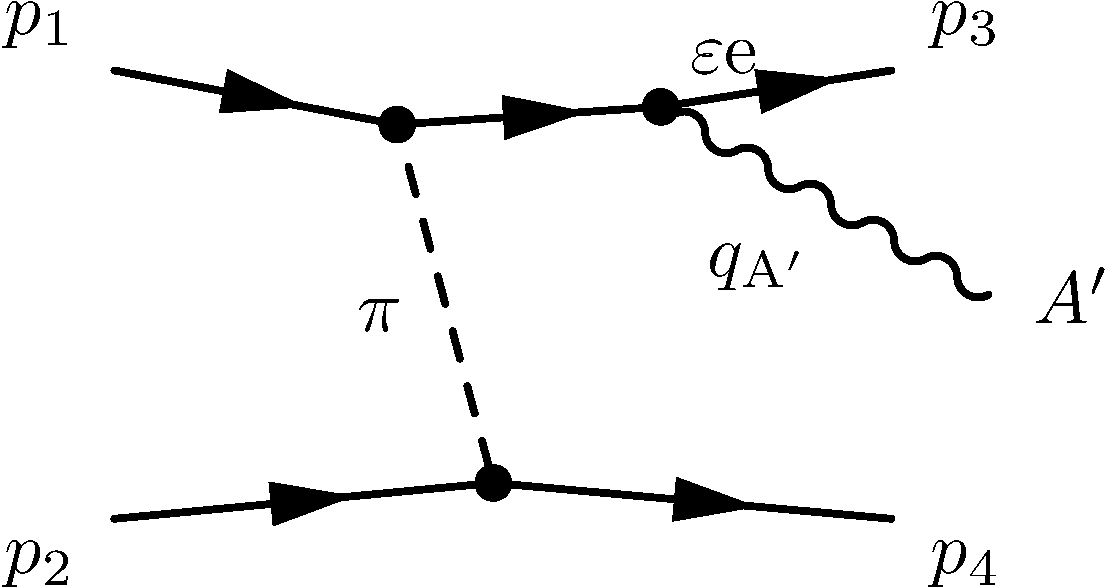
\includegraphics[width=8cm]{ppdiagram.pdf}
\caption{One of the eight Feynman diagrams for the pp process. Three of the other diagrams are obtained by 
placing the $A'$ on each of the protons in turn. The remaining four diagrams come from swapping the outgoing 
momenta.}
\label{fig:ppdiagram}
\end{figure}
	
Evaluating these diagrams is tedious, but very straightforward. The calculation differs 
from the well-known axion bremsstrahlung calculation, because the mass of the $A'$ boson is not 
necessarily negligible in the kinematic region of interest for supernova explosions.
The correct kinematical relations are 
%
\bea 
p_1 \cdot p_2 &=& M_N^2 - \frac{l^2}{2} - \frac{k^2}{2} + p_2 \cdot \qa,\\
p_1 \cdot p_3 &=& M_N^2 + k \cdot l - \frac{k^2}{2} + p_3 \cdot \qa,\\  
p_1 \cdot p_4 &=& k \cdot l + M_N^2 - \frac{l^2}{2} + p_4 \cdot \qa, \\
p_2 \cdot p_3 &=& M_N^2 - \frac{l^2}{2}, \\ 
p_2 \cdot p_4 &=& M_N^2 - \frac{k^2}{2},\quad \mathrm{and}\\
p_3 \cdot p_4 &=& k \cdot l + M_N^2 - \frac{l^2 + k^2}{2},
\eea
%
where $p_1$ and $p_2$ are the four-momenta of the incoming nucleons, $p_3$ and $p_4$ are the momenta 
of the outgoing nucleons, $\qa$ is the $A'$ momentum, $k=p_2 - p_3$, $l=p_2 - p_4$, and $M_{\mathrm{N}}$ 
is the nucleon mass. These kinematical relations correct the relations in Ref.~\cite{dent_etal12}.

\arz{Cameron, can you double check this. I think there were some errors in the momenta and in the relative 
signs of the diagrams. I tried to fixe them.}
The eight diagrams contribute the following eight terms to the pp amplitude, 
%
\begin{widetext}
\begin{eqnarray}
	M_1 &=& \frac{4 M_N}{ m_\pi} \frac{f_{pp}^2 e \varepsilon}{k^2-m_\pi^2}  \frac{1}{m_{A^\prime}^2 - 2 \qa \cdot p_1} 
	\bar{u}(p_4) \gamma_5 u(p_2) \bar{u}(p_3) \gamma_5 (\slashed{p}_1 - \qa +M_N)\slashed \epsilon  u(p_1), \\
	M_2 &=& -\frac{4 M_N}{ m_\pi} \frac{f_{pp}^2 e \varepsilon}{l^2-m_\pi^2}  \frac{1}{m_{A^\prime}^2 - 2 \qa \cdot p_1} 
	\bar{u}(p_3) \gamma_5 u(p_2) \bar{u}(p_4) \gamma_5 (\slashed{p}_1 - \qa +M_N)\slashed{\epsilon} u(p_1),\\
	M_3 &=& \frac{4 M_N}{ m_\pi} \frac{f_{pp}^2 e \varepsilon}{l^2-m_\pi^2}  \frac{1}{m_{A^\prime}^2 - 2 \qa \cdot p_2} 
	\bar{u}(p_3) \gamma_5 u(p_1) \bar{u}(p_4) \gamma_5 (\slashed{p}_2 - \qa +M_N)\slashed \epsilon  u(p_2), \\
	M_4 &=& -\frac{4 M_N}{ m_\pi} \frac{f_{pp}^2 e \varepsilon}{k^2-m_\pi^2}  \frac{1}{m_{A^\prime}^2 - 2 \qa \cdot p_2} 
	\bar{u}(p_4) \gamma_5 u(p_1) \bar{u}(p_3) \gamma_5 (\slashed{p}_2 - \qa +M_N)\slashed \epsilon  u(p_2), \\
	M_5 &=& \frac{4 M_N}{ m_\pi} \frac{f_{pp}^2 e \varepsilon}{k^2-m_\pi^2}  \frac{1}{m_{A^\prime}^2 + 2 \qa \cdot p_3} 
	\bar{u}(p_3) \gamma_5 u(p_1) \bar{u}(p_4) \slashed{\epsilon} (\slashed{p}_3 + \qa +M_N)\gamma_5 u(p_2),\\
	M_6 &=& -\frac{4 M_N}{ m_\pi} \frac{f_{pp}^2 e \varepsilon}{l^2-m_\pi^2}  \frac{1}{m_{A^\prime}^2 + 2 \qa \cdot p_3} 
	\bar{u}(p_4) \gamma_5 u(p_1) \bar{u}(p_3) \slashed{\epsilon} (\slashed{p}_3 + \qa +M_N)\gamma_5 u(p_2),\\
	M_7 &=& \frac{4 M_N}{ m_\pi} \frac{f_{pp}^2 e \varepsilon}{k^2-m_\pi^2}  \frac{1}{m_{A^\prime}^2 + 2 \qa \cdot p_4} 
	\bar{u}(p_4) \gamma_5 u(p_2) \bar{u}(p_3) \slashed{\epsilon} (\slashed{p}_4 + \qa +M_N)\gamma_5 u(p_1),\\
	M_8 &=& -\frac{4 M_N}{ m_\pi} \frac{f_{pp}^2 e \varepsilon}{l^2-m_\pi^2}  \frac{1}{m_{A^\prime}^2 + 2 \qa \cdot p_4} 
	\bar{u}(p_3) \gamma_5 u(p_2) \bar{u}(p_4) \slashed{\epsilon} (\slashed{p}_4 + \qa +M_N)\gamma_5 u(p_1),
\end{eqnarray}
\end{widetext}
%
where the dark photon polarization is given by $\epsilon$. The squared amplitude is given by 
%
\begin{equation}
\vert \mathcal{M}_{\mathrm{pp}} \vert^2 = \sum_{s_1,s_2}\, \left\vert \sum_{i=1}^{8}\, M_i \right\vert^2, 
\end{equation}
%
where the first summation is over the incoming proton polarizations. These expressions are identical to those 
given in Ref.~\cite{dent_etal12}; however, they do not simplify significantly if the correct kinematics are used. 
Unfortunately, with the kinematical relations above, the squared amplitude does not yield a tidy expression 
for the spin-averaged squared matrix element. Our result 
contains over 200 terms, so we do not reproduce it here for reasons of convenience. However, we note that 
our result for $\vert \mathcal{M}_{\mathrm{pp}} \vert^2$ is symmetric under exchange of $k$ and $l$ as required. 

The pn process contain four diagrams analogous to the the diagrams for the pp process (there are only four, of course, 
because the neutrons cannot radiate the $A'$). The new diagram that is relevant in the pn process is shown in 
Fig.~\ref{fig:npdiagram} and yields a contribution of 
%
\begin{widetext}
\begin{equation}
M'_5 = \frac{4 M_N}{ m_\pi} \frac{f_{pn}^2 e \varepsilon}{l^2-m_\pi^2}  \frac{1}{(l-\qa)^2 - m_\pi^2} 
\bar{u}(p_3) \gamma_5 u(p_1) \bar{u}(p_4) \gamma_5 u(p_2) (\qa - 2l)\cdot \varepsilon.
\end{equation}
\end{widetext}
%
The pn processes likewise yield a squared amplitude, 
$\vert \mathcal{M}_{\mathrm{pn}} \vert^2$ that is unwieldy, so we do not give the 
the full expression here. 


%-------------- NP Feynman Diagram
\begin{figure}
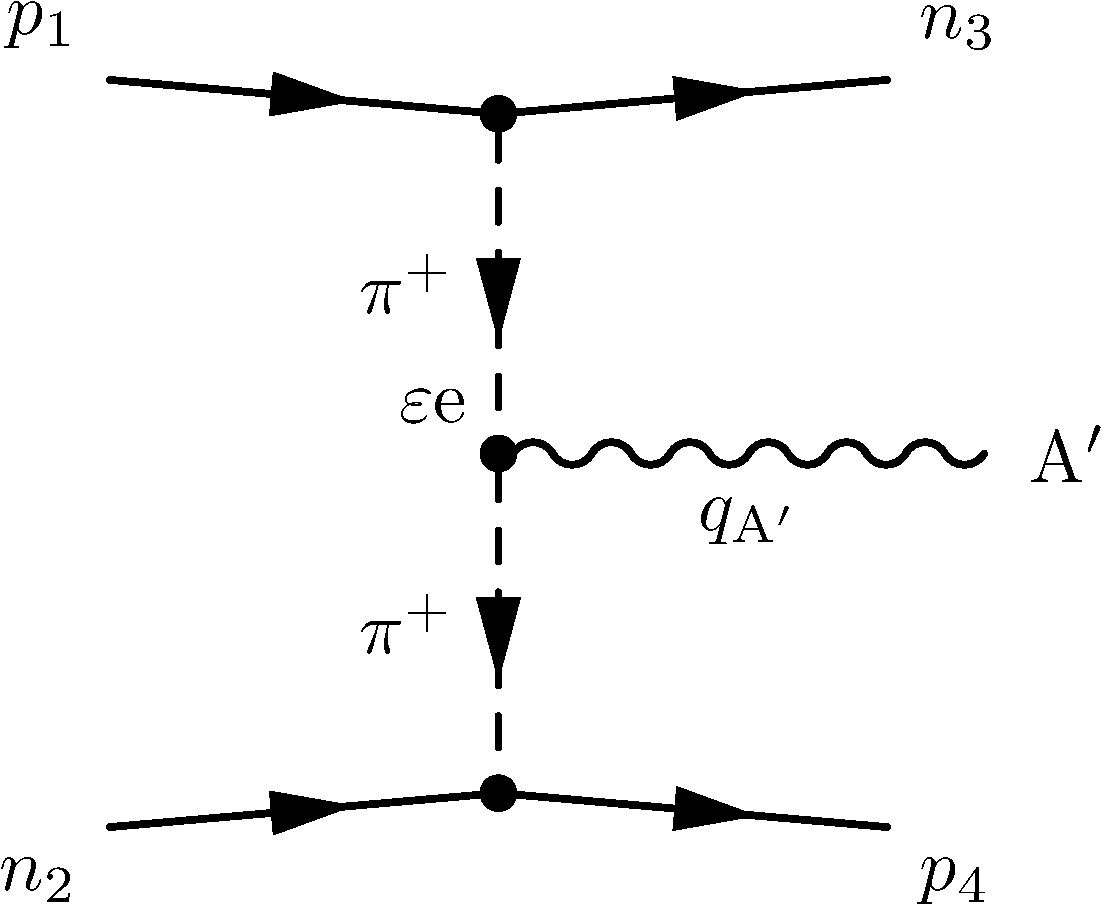
\includegraphics[width=8cm]{npdiagram.pdf}
\caption{One of the five Feynman diagrams for the np process. This particular diagram shows 
internal brehmsstrahlung off of the charged pion. The remaining four diagrams are analogous to the 
pp diagram shown in Fig.~\ref{fig:ppdiagram}.}
\label{fig:npdiagram}
\end{figure}


%------------------------------------- STREAMING CONSTRAINT
\subsection{The Streaming Limit of the Energy Loss Rate}

The first and simplest bound that may be obtained arises from assuming that all $A'$ particles produced in the supernova core 
leave the supernova, carrying their energies with them. The constraint can be derived simply by 
requiring that the energy loss through this cooling channel be less than the cooling from neutrino emission; 
any greater, and it would have an observable effect on supernova cooling. This calculation yields values of 
$\varepsilon$ above which cooling through $A'$ production is too rapid to be consistent with SN1987A. 
We will consider modifications to this bound from $A'$ trapping and decay in subsequent subsections.

The quantity of interest is the rate of energy emission through dark gauge bosons. 
From the spin-summed, squared amplitudes described in the previous subsection, 
the energy emission rate is obtained by integrating over the phase space, 
and adding a factor of the energy of the emitted particle. To be specific, the 
energy emission rate per unit volume is 
%
\begin{widetext}
\beq
\label{eq:rate1}
Q_i = (2\pi)^4 \int\, E_{\mathrm{A}'} \, \sum_{s_1,s_2}\, \vert \mathcal{M}_i \vert^2 f(p_1) f(p_2)\delta^{(4)}(p_1+p_2-p_3-p_4-\qa)\, d\Pi,
\eeq
\end{widetext}
%
where $d\Pi$ is the Lorentz-invariant phase space, 
$ E_{\mathrm{A}'}$ is the energy of the emitted $A'$ boson, 
$f(p)$ are the phase-space densities of the incoming nucleons, and 
the index $i$ refers to either the pp or pn processes. 
The nucleons in the core are comfortably non-degenerate and non-relativistic, 
so the Pauli blocking factor is omitted from Eq.~(\ref{eq:rate1}) and we take 
all nucleons to have a Maxwell-Boltzmann momentum distribution, so 
\beq
f(p) =  \frac{n_b}{2} \left( \frac{2 \pi}{M_N T} \right)^{3/2} \exp \left(-\frac{p^2}{2 M_N T} \right).
\eeq
%
We chose a baryon number density of $n_{\mathrm{b}} \approx 1.8 \times 10^{38}\, \mathrm{cm}^{-3}$ and a 
core supernova temperature of $T = 30\, \mathrm{MeV}$, both of which are typical choices and thought to 
be representative of supernova cores. \arz{Need to put a citation here for the properties of supernova cores. 
I can probably find something in the literature, but please put something here if you have a citation.}

We performed the phase space integrals using the Monte Carlo routines in the {\tt CUBA} library. 
\arz{There needs to be some reference, citation, or some other information give about this library here.} 
We integrated over the momenta $\vec{p}_1$, $\vec{p}_2$, $\vec{p}_3$, and the direction of the 
three-momentum of the radiated boson $\hat{q}_{\mathrm{A}'}$, after fixing $\vec{p}_4$ 
and the magnitude of $\vec{q}_{\mathrm{A}'}$ using the delta functions. 
\arz{Cameron, can you double check this to be sure that it is correct? I rephrased it a bit, 
but I found the earlier phrasing to be a bit ambiguous and I can't remember which choice 
you made.} We used the {\tt suave} method provided within {\tt CUBA}, which combines 
importance sampling and adaptive subdivision, as this method provided the best compromise 
between accuracy and run-time for this particular application.

To obtain the dark gauge boson luminosity from $Q_{\mathrm{pp}}$ and $Q_{\mathrm{pn}}$, 
we assumed that $A'$ production takes place in a stellar core of radius $\sim 1$~km, so that 
the total luminosity of $A'$ is 
%
\begin{equation}
L_{\mathrm{A}'} = V (Q_{\mathrm{pp}} + Q_{\mathrm{pn}})
\end{equation}
%
where $V$ is the volume of the sphere. Clearly, $L_{\mathrm{A}'}$ is proportional to $\varepsilon^2$, 
so that writing $L_{\mathrm{A}'} = \varepsilon^2 I_{\mathrm{A}'}(m_{\mathrm{A}'},T)$ and 
$L_{\nu}$ as the neutrino luminosity, we can write the constraint as 
%
\begin{equation}
\varepsilon \lesssim \sqrt{\frac{L_{\nu}}{I_{\mathrm{A}'}(m_{\mathrm{A}'}, T)}}.
\end{equation}
%
Following SOMEBODAY \arz{We need a citation here.}, we show a constraint taking 
$L_{\nu} \approx 10^{53}\, \mathrm{erg/s} \approx 4 \times 10^{37}\, \mathrm{MeV}^2$. 

%---------------------------------- DECAY LIMIT
\subsection{Decay limit}
The constraint from the streaming limit above provides an upper bound on the allowed coupling (or lower bound on the excluded coupling) by considering the production on the $A'$. Naively it might be expected that this suffices, in that all higher couplings are excluded. However, in order to function as a cooling channel, enough of the produced dark gauge bosons must escape the supernova. As the coupling increases, so do processes that prevent the escape, and so the excluded region has an upper bound, above which the luminosity again drops below the neutrino luminosity. The first such limit may be found by considering decay of the dark bosons into Standard Model particles, and assuming that these SM particles are trapped in the supernova core and contribute nothing to the cooling. The dark boson has a typical lifetime of 
\beq
l = \frac{3 E_{A}}{N_{eff} m_A^2 \varepsilon^2},
\eeq
and so the fraction escaping the supernova before decaying is given by 
\beq
e^{r_{decay}/l} = e^{r_{decay} N_{eff} m_A^2 \varepsilon^2/(3 E_A)}.
\eeq
To take this into account, the above exponential factor is simply appended to the phase space integrand, and the calculation then proceeds as before. The limit is derived from the same equation, with the only complication being the fact that $ I_A $ is now a function of $ \varepsilon $, in addition to $ m_A, T $. This makes the numerical calculation slightly more complicated, but otherwise changes nothing of importance, with now the constraint a transcendental equation,  
\beq
\varepsilon \le \sqrt{\frac{4.1 \times 10^{37} MeV^2}{I_A(m_A, T, \varepsilon)}}.
\eeq
	

%---------------------------------- TRAPPING	
\subsection{Trapping limit}
The second constraint that produces an upper bound on the excluded region comes from considering trapping of dark bosons within the supernova. With a large enough coupling, the new particles will thermalize and then will be emitted from a spherical shell.  In this case the luminosity is given simply by the Steffan-Boltzmann law
\beq
\mathcal{L}_t  = 4\pi r^2 T_A^4 \sigma,
\eeq
where $ r $ is now the radius of the emitting shell and $ T_A $ its temperature. We can estimate $ r = 10$ km, since the density of the supernova drops drastically around that point. After taking that value for r, the bound on the luminosity translates into a bound on $ T_A $ 
\beq
T_A \le 9.586\rm\ MeV.
\eeq
That bound can then be translated into the desired bound on the coupling as a function of mass by assuming that the particles are emitted from an optical depth $ \tau = 2/3 $, and finding the temperature that corresponds to that optical depth. This is a somewhat involved calculation.
First, one needs a model for the density and temperature in the supernova. Following \cite{dent_etal12}, we assume 
\bea
\rho &=& \rho_p \left(\frac{R}{r}\right)^n,\\
T &=& T_R \left(\frac{\rho(r)}{\rho_R}\right)^{1/3},
\eea
with $  \rho_p  = 3\times10^{14}\ {\rm g/cm}^3, T_R = 30$ MeV, and taking $ n = 5 $. The optical depth is given by 
\beq
\tau = \int_{r_x}^{\infty} \kappa \rho dr,
\eeq
where $ \kappa$ is the opacity.  To find the opacity, we start from the reduced mean Rosseland opacity 
\beq
\frac{1}{\kappa \rho} = \int_{m_x}^{\infty} \frac{15}{4 \pi^4 T^5} \frac{E_A^2 e^{E_A/T} \sqrt{E_A^2 - m_A^2}}{(e^{E_A/T}-1)^2} l_A dE_A,
\eeq
where $ l_A $ is the mean free path. 
	
The inverse mean free path can readily be obtained by modifying $ Q_i $, the expression for the energy loss rate, as follows: removing the factor of $ E_A $ and the phase space integral over $ \qa $, and adding a factor of $ e^{E_A/T} $ for detailed balance. This gives the inverse mean free path as a function of mass and coupling. Again the required integration is performed numerically. This then allows the calculation of $ \kappa_x $. The inverse opacities for the $pn$ and $pp$ processes add, giving the total opacity $ \kappa^{-1} = \kappa_{pp}^{-1} + \kappa_{pn}^{-1} $
	
Having obtained an expression for $ \kappa $, we can now find the optical depth as follows: define a new quantity $ \tau_R = \kappa_R \rho_R R $. We then have 
\beq \kappa \rho R = \tau_R (\frac{\rho}{\rho_R})^2 (\frac{T_R}{T})^{3/2}  \eeq
This is combined with the expressions for the density and temperature as a function of r and plugged in to the integral expression for the optical depth to obtain 
\bea \tau_x &=& \int_{r_x}^{\infty} \tau_R (\frac{R}{r})^{3n/2} \\
 &=& \frac{\tau_r}{\frac{3n}{2}-1} (\frac{T_A}{T_R})^{(9/2-3/n)} \eea
and the bound on the coupling is finally found by requiring  $ \tau_x(\varepsilon,m_A) \le 2/3 $
	
	
	
\subsection{Phase Space Integration}

In every case 	

Once the integration is complete the calculation of the trapping and streaming limits is a straightforward application of the equations previously derived, and proceeded as outlined above. The decay limit is somewhat harder, since $ \varepsilon $ appears on both sides of the equation. Again we employed an unsubtle approach to solving the problem: $ \varepsilon $ was set to an arbitrary value where the constraint was satisfied, and then iteratively reduced until the constraint was no longer satisfied. This obviously introduces another source of error, but with a sufficiently small interval in $ \varepsilon $ this is negligible. The one further slight complication is that at after a certain value of $ M_A $ the decay limit rapidly goes to zero, at which point the procedure was terminated.
	



%-------------------- RESULTS
\section{Results}
\label{section:results}

\begin{figure}[th]
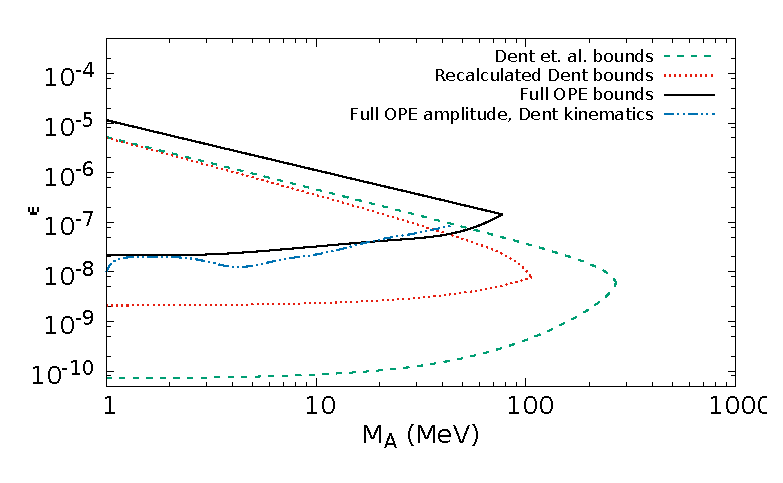
\includegraphics[width=9cm]{stages.eps}
\caption{The changes in the bounds generated as each stage of the calculation departs from Ref.~\cite{dent_etal12}. Interestingly the kinematics have apparently relatively little effect.
\arz{Cameron, several to-do items for this figure. On the y-axis, the symbol should be "$\varepsilon$" rather than 
"e". Can we write numbers as "$10^{-9}$" rather than "1e-09" and so on? Can we make the axis labels and 
tick mark labels larger? Can you make all of the lines thicker? Can you make each of the four lines a distinct color?}
}
\end{figure}

Let's put some text here.

\begin{figure}[th]
	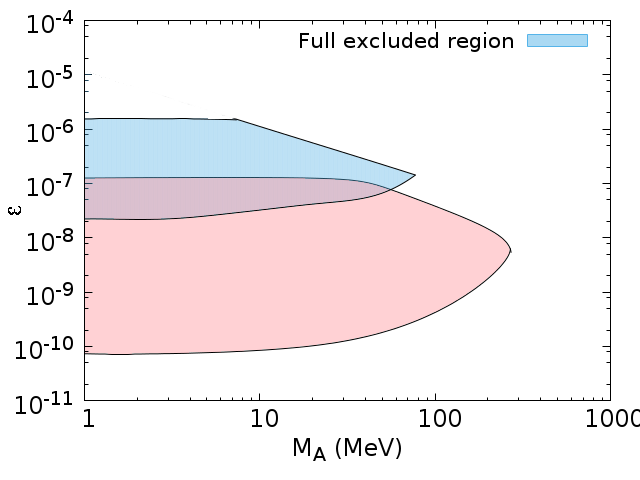
\includegraphics[width=9cm]{endtoend.png}
	\caption{A comparison of the final result for the excluded region with the result from Ref.~\cite{dent_etal12}. The excluded region is clearly significantly less restrictive, and opens up the region of parameter space for $\varepsilon \approx  1e-8-9 $.
\arz{Cameron, some similar comments as for Figure 1. Can we write numbers as "$10^{-9}$" rather 
than "1e-09" and so on? Can we make the axis labels and tick mark labels larger?}	
	}
\end{figure}


%--------------------------- CONCLUSIONS
\section{Discussion and Conclusions}
\label{section:conclusions}


	The revised approach produce constraints that are significantly weaker than the previous work, and that largely reproduce constraints already obtained from beam dump experiments. 




\acknowledgments

AKL was supported in part by NSF grant PHY-1519175.


\bibliography{draft}

\end{document}

%%%%%%%%%%%%%%%%%%%%%%%%%%%%%%%%%%%%%%%%%%%%%%%%%%%%%%%%%%%%%%%%%%%%%%
%%%%%%%%%%%%%%%%%%%%%%%%%%%%% Bibliography %%%%%%%%%%%%%%%%%%%%%%%%%%%
%%%%%%%%%%%%%%%%%%%%%%%%%%%%%%%%%%%%%%%%%%%%%%%%%%%%%%%%%%%%%%%%%%%%%%


%%%%%%%%%%%%%%%%%%%%%%%%%%%%%%%%%%%%%%%%%%%%%%%%%%%%%%%%%%%%%%%%%%%%%%

\end{document}